% !TeX spellcheck = en_US

\chapter{Technical Foundations}
\label{ch:tech}

This chapter provides additional technical details for specific algorithms and techniques that are later referenced in our System Design (Chapter~\ref{ch:system}). Feel free to skip this chapter if you are roughly familiar with the following methods: $2D$ object instance segmentation, the \textit{OpenDRIVE} and \textit{Lanelet2} map data formats, the \textit{Robot Operating System (ROS)}, the \textit{DBSCAN} point clustering algorithm, the \textit{SORT} object tracking algorithm, the \textit{L-Shape-Fitting} algorithm (as previously mentioned in Section~\ref{sec:related-lshape-fitting}), and common object detection evaluation metrics, such as \textit{mAP} and \textit{IoU}.

\section{The YOLACT Instance Segmentation Model}
\label{sec:yolact}

\textit{YOLACT (You Only Look At Coefficients)}~\cite{bolya2019yolact} is a real-time instance segmentation method that focuses on processing static images.
It simplifies the instance segmentation problem by separating it into two parallel tasks, enabling faster processing while maintaining competitive accuracy.
The functionality of \textit{YOLACT} can be described in three main steps (as illustrated in Figure~\ref{fig:yolact}):

\begin{enumerate}
    \item \textbf{Generating Prototype Masks:} \textit{YOLACT} employs a fully convolutional network called \textit{ProtoNet} to generate a fixed set of K prototype masks, which are used as the base for constructing the final object instance masks.\ These prototype masks are shared across all object instances in the image.
    \item \textbf{Predicting Per-instance Mask Coefficients and Bounding Boxes:} In parallel to generating prototype masks, \textit{YOLACT} predicts per-instance mask coefficients and bounding boxes for potential objects using an anchor-based approach.\ Each anchor is associated with a mask coefficient vector, which has the same length as the number of prototype masks (K). Additionally, the model predicts the class probabilities and bounding box coordinates for each anchor.
    \item \textbf{Assembling Final Instance Masks:} To obtain the final instance masks, \textit{YOLACT} linearly combines the prototype masks using the predicted mask coefficients.\ The model selects the top scoring instances based on their class probabilities and applies a non-maximum suppression (NMS) algorithm to remove duplicate detections.\ The result is a set of instance masks, each associated with a specific object class and bounding box.
\end{enumerate}

\textit{YOLACT's} architecture consists of a feature backbone (e.g., \textit{ResNet}~\cite{targ2016resnet} or \textit{MobileNet}~\cite{howard2017mobilenets}), a Feature Pyramid Network (FPN) for multiscale feature extraction, and separate prediction heads for class, bounding box, and mask coefficients.
This architecture allows it to achieve real-time instance segmentation on static images, with a good balance between speed and accuracy.
However, it is designed for large GPUs, such as the \textit{TitanX} or \textit{RTX-2080-Ti}, and its performance on lower-power edge devices is limited without further optimization or adaptations, which is where \textit{YolactEdge}~\cite{liu2021yolactedge} comes in to address these limitations.

\begin{figure}[htb]
    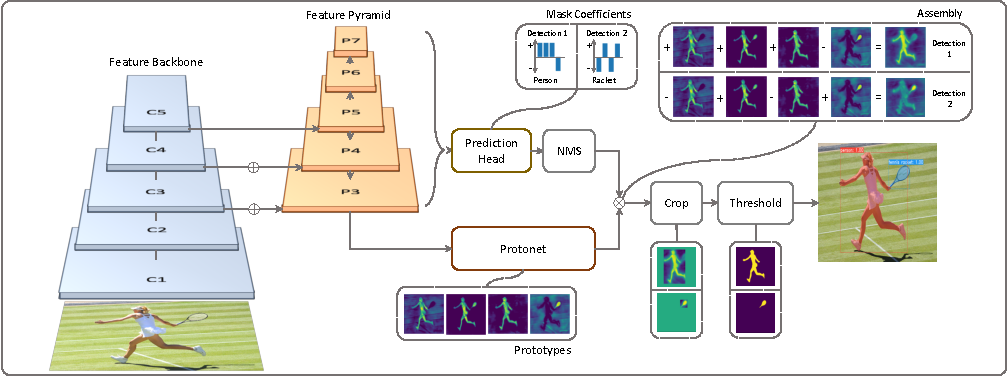
\includegraphics[width=\linewidth]{figures/yolact_fig_2-cropped}
    \caption{Figure~2 from \textit{YOLACT}. The figure shows how generated protorype masks are combined with instance-specific coefficients to produce the final instance masks.}
    \label{fig:yolact}
\end{figure}

\textit{YolactEdge} is a real-time instance segmentation method designed for edge devices, focusing on video processing.
Its functionality can be broken down into two main improvements over the original \textit{YOLACT} method:

\begin{enumerate}
    \item \textbf{\textit{TensorRT} Optimization:} \textit{YolactEdge} utilizes NVIDIA's \textit{TensorRT}~\cite{vanholder2016efficient} inference engine to optimize the neural network.\ \textit{TensorRT} provides mixed-precision support, optimal tensor layout, layer fusion, and kernel specializations.\ It quantizes model weights to \texttt{INT8} or \texttt{FP16} precision, which can speed up the processing while preserving accuracy.\ \textit{YolactEdge} explores the optimal mix between INT8 and FP16 weights for different model components, maximizing speed without significant degradation in accuracy.\ The \textit{TensorRT} optimization results in around a 4x improvement in speed when working with static images.
    \item \textbf{Exploiting Temporal Redundancy in Video:} \textit{YolactEdge} takes advantage of the temporal redundancy in videos, which means that neighboring frames in a video sequence are often highly correlated.\ Instead of computing expensive backbone features for every frame, YolactEdge divides the frames into two groups: keyframes and non-keyframes.\ For keyframes, the model computes all backbone and pyramid features.\ For non-keyframes, only a subset of features is computed, while the rest are transformed from the temporally closest previous keyframe.
\end{enumerate}

By combining \textit{TensorRT} optimization and exploiting temporal redundancy, YolactEdge can achieve real-time instance segmentation on edge devices such as Jetson AGX Xavier with a high frame rate and competitive accuracy.
This makes it an ideal solution for applications like robotics, autonomous driving, security, and augmented reality that require real-time processing and low latency.

\section{The YOLOv7 Instance Segmentation Model}
\label{sec:yolovseven}

\textit{YOLOv7}~\cite{wang2022yolov7}, as a state-of-the-art real-time object detection model, demonstrates significant quantitative improvements in object detection performance.
It not only excels in this primary task but also showcases its adaptability and effectiveness in related computer vision tasks, such as instance segmentation.

To achieve high-performance real-time instance segmentation, \textit{YOLOv7} is integrated with BlendMask, a technique introduced in the paper \enquote{BlendMask: Top-Down Meets Bottom-Up for Instance Segmentation}.
BlendMask builds upon the foundation laid by \textit{YOLACT}, but with a key difference in its approach to blending masks within bounding boxes.
While \textit{YOLACT} predicts a single scalar coefficient for each prototype mask, BlendMask predicts a low-resolution $(7*7)$ attention map for the same purpose, as described in Figure~\ref{fig:blendmask}.

\begin{figure}[htb]
    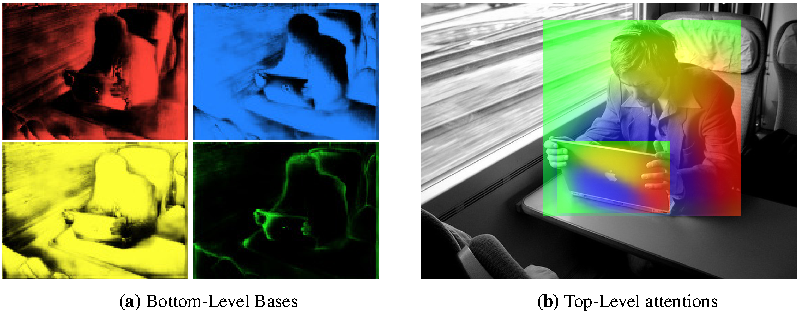
\includegraphics[width=\linewidth]{figures/blendmask_fig_3-cropped}
    \caption{Figure~3 from \textit{BlendMask}, showcasing how it replaces \textit{YOLACT's} Prototype Masks with Bottom-Level Bases which are combined using per-instance Top-Level Attention maps rather than coefficients.}
    \label{fig:blendmask}
\end{figure}

This attention map, which functions as a high-dimensional feature, is attached to each bounding box.
The blending of masks using the attention map results in a more precise and refined instance segmentation.
To leverage \textit{YOLOv7} for instance segmentation, the \textit{YOLOv7} object detection model is fine-tuned on the \textit{MS COCO}~\cite{lin2014microsoft} instance segmentation dataset.
The resulting \textit{YOLOv7}-mask model achieves a Mask AP (average precision) of $43.1\%$, while \textit{YOLACT} achieves a Mask AP of $35.4\%$ when using a \textit{ResNet-101} backbone.
The architecture of \textit{YOLOv7}-mask, as well as some of the qualitative corresponding results, are illustrated in Figure XXX.

% ----------------------------------------------------

\section{Map Data Formats}
\label{sec:opendrive}

This work depends on HD maps to inform viable heading heading choices for road user detections.
As map data formats for this task, both the \textit{OpenDRIVE}~\cite{dupuis2010opendrive, althoff2018automatic} and \textit{Lanelet2}~\cite{poggenhans2018lanelet2} map data formats are considered.
In both \textit{OpenDRIVE} and \textit{Lanelet2} formats, lane geometry representation is crucial for accurate road modeling and navigation.
\textit{OpenDRIVE} is an XML-based data format that describes road networks hierarchically.
It consists of roads, lanes, junctions, objects, and signals, with each road having a unique identifier and geometric information.
Lanes are classified into driving lanes, sidewalks, and shoulders, while junctions define connections between roads.
\textit{Lanelet2}, on the other hand, uses a combination of XML and OSM formats for data representation.
It is based on the concept of \enquote{lanelets}, which are individual driving lanes with associated traffic rules.
\textit{Lanelet2} includes left and right boundaries, regulatory elements, and routing graphs.

In \textit{OpenDRIVE}, lane geometry is represented using a combination of planar and lateral geometric information.
The geometry of a road is defined by a reference line, which is a parametric curve.
This curve is specified using a series of points and can be described by different types of geometry, such as straight lines, spirals, arcs, and clothoids.
The reference line represents the road's centerline, and the lanes are defined relative to it.
Lanes in \textit{OpenDRIVE} are divided into three categories: driving lanes, sidewalks, and shoulders.
Each lane has attributes such as width, type, and road marks.
The lateral position of a lane is described by a set of functions, which determine the lane's width as a function of its longitudinal position along the road.
This information, along with the road's reference line, is used to compute the geometry of individual lanes.

\textit{Lanelet2} uses a simpler approach for representing lane geometry.
It employs polygons, with each lanelet defined as a drivable polygon consisting of left and right boundaries.
The boundaries are sequences of nodes (points with longitude and latitude), which form linear or curved segments.
The nodes are ordered along the lanelet's direction, and the shape of the lanelet is derived by connecting corresponding nodes from the left and right boundaries.
Lane boundaries in \textit{Lanelet2} can be solid or dashed lines, indicating whether lane changes are allowed.
Unlike \textit{OpenDRIVE}, which uses parametric curves for defining road geometry, \textit{Lanelet2} uses a more straightforward representation based on sequences of points.
This approach can be less accurate in some cases, but it simplifies map data handling and provides better compatibility with OpenStreetMap data.

\begin{figure}[htb]
    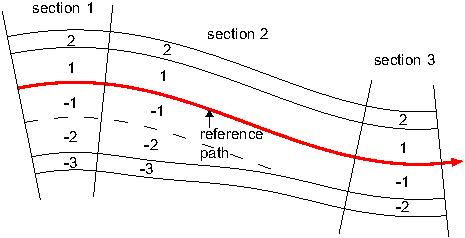
\includegraphics[width=0.49 \linewidth]{figures/opendrive_to_lanelet_fig_2_-cropped}
    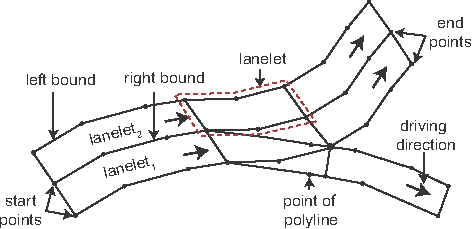
\includegraphics[width=0.49 \linewidth]{figures/opendrive_to_lanelet_fig_3-cropped}
    \caption{Figures~2 and~3 from~\cite{althoff2018automatic}. The left-hand-side image shows a typical \textit{OpenDRIVE}-based model with multiple lane-sections based on a common continuous reference line. The left-hand-side image shows the simpler modeling approach of \textit{Lanelet2}, where lanes are based on self-contained pre-triangulated shapes.}
    \label{fig:opendrive-lanlet}
\end{figure}

In summary, \textit{OpenDRIVE} represents lane geometry using parametric curves and a reference line, while \textit{Lanelet2} uses polygonal shapes defined by sequences of nodes.
\textit{OpenDRIVE} offers more accurate road geometry, but \textit{Lanelet2's} simpler representation can be easier to work with and integrate with other mapping data sources like OpenStreetMap. This modeling difference is also highlighted in Figure~\ref{fig:opendrive-lanlet}.
In this work, we are compelled to use \textit{OpenDRIVE} as the input format for the HD map, as this format was used by Providentia's map data supplier.
However, the \textit{Lanelet2} format would be more suitable, as their approach to lane modeling is directly compatible with our heading interpolation algorithm, as described in Section~\ref{sec:hdmapgrids}.

% ----------------------------------------------------

\section{The Robot Operating System}
\label{sec:ros}

The \textit{Robot Operating System (ROS)}~\cite{quigley2009ros} is a flexible software framework for developing robotic applications.
Its main goal is to simplify the creation of complex and robust robot behavior across various platforms.

\textit{ROS} follows a graph architecture, where modular components called nodes communicate with one another through a publish-subscribe messaging model.
Nodes are single-purpose components responsible for specific tasks, such as controlling a sensor or processing data.
They exchange information by sending messages over named channels called \textit{topics}.
Another central component in \textit{ROS} is the Master, which manages the entire system by allowing nodes to find each other, register topics and services, and maintain a list of active nodes.

The framework provides several advantages for robotics applications, including hardware abstraction, low-level device control, efficient message passing, package management, and a rich ecosystem of tools and libraries.
These features make it easier for developers to build distributed robotics applications, and promote modularity and code reusability.
In our case, we divide separate detector stages into different nodes, as described in Section~\ref{sec:arch}.

\section{SORT Object Tracking}
\label{sec:sort}

The \textit{Simple Online and Realtime Tracking (SORT)}~\cite{bewley2016simple} algorithm is an object tracking method that is specifically designed for tracking multiple objects in real-time.
It employs a combination of detection and tracking to maintain the identity of objects as they move across video frames.
\textit{SORT} is lightweight and computationally efficient, making it suitable for real-time applications.

At the core of the \textit{SORT} algorithm is the \textit{Kalman Filter}~\cite{welch1995kalman}, a recursive estimation technique that helps to predict the state of a dynamic system over time, even in the presence of noise.
In the context of object tracking, the \textit{Kalman Filter} is used to estimate the position, velocity, and other parameters of objects in the video frames.

Here is a step-by-step description of the \textit{SORT} algorithm and its use of \textit{Kalman Filters}:

\begin{enumerate}
    \item \textbf{Object Detection:} First, an object detection algorithm, such as YOLO (You Only Look Once) or Faster R-CNN, is applied to the input video frames to identify objects of interest and generate bounding box coordinates for each detected object.
    \item \textbf{Initialization:} For each detected object, a \textit{Kalman Filter} is initialized with the bounding box coordinates as the initial state.\ The state vector typically includes the position $(x, y)$ and velocity $(vx, vy)$ of the object's center.\ Additionally, a unique ID is assigned to each object.
    \item \textbf{Prediction:} For each object, the \textit{Kalman Filter} predicts its state in the next frame.\ This is done by applying a state transition model to the current state, which usually involves updating the position based on the velocity.
    \item \textbf{Data Association:} In the subsequent frame, the newly detected objects are matched with the predicted states of the existing tracked objects.\ This association is achieved using a distance metric, typically the Intersection over Union (IoU) or the Mahalanobis distance.\ A bipartite graph matching algorithm, such as the Hungarian algorithm~\cite{kuhn1955hungarian}, is employed to find the optimal assignment between detections and tracked objects.
    \item \textbf{Update:} Once the data association is completed, the \textit{Kalman Filter} is updated with the new measurements (bounding box coordinates) of the associated detected objects.\ This step incorporates the new observations into the existing state estimate, considering both the prediction and the measurement uncertainties.
    \item \textbf{Handling Occlusions and New Objects:} If a tracked object is not detected in the new frame, its \textit{Kalman Filter's} state is still updated based on the prediction alone.\ If an object is missing for a certain number of consecutive frames, it is removed from the tracking list.\ Conversely, if a new object is detected, a new \textit{Kalman Filter} is initialized and added to the tracking list.
    \item \textbf{Output:} The final output of the \textit{SORT} algorithm is a list of tracked objects, each with a unique ID and an updated bounding box for each frame.
\end{enumerate}

In summary, the \textit{SORT} algorithm uses \textit{Kalman Filters} to predict and update the state of objects in a video sequence, maintaining their identities while tracking their positions and velocities over time.\ The data association step ensures that the correct detections are matched with the corresponding tracked objects, making the tracking robust and efficient.

% ----------------------------------------------------

\section{The DBSCAN Algorithm}
\label{sec:dbscan}

\textit{DBSCAN}, which stands for \textit{Density-Based Spatial Clustering of Applications with Noise}~\cite{schubert2017dbscan}, is a popular unsupervised machine learning algorithm designed for cluster analysis.
It works by identifying dense regions in the input data, separating them into distinct clusters, and treating low-density regions as noise.

\textit{DBSCAN} has the following key functionalities:

\begin{enumerate}
    \item \textbf{Density-based clustering:} The algorithm groups data points based on their density in the feature space.\ A dense region is defined as an area with a high concentration of data points, while a low-density region has fewer data points.
    \item \textbf{Automatic detection of the number of clusters:} Unlike some other clustering algorithms, like K-means, \textit{DBSCAN} does not require the user to specify the number of clusters beforehand.\ The algorithm automatically determines the number of clusters based on the input data.
    \item \textbf{Robustness to noise:} \textit{DBSCAN} can identify and separate noise from the data.\ Noise is defined as data points that do not belong to any dense region and are not part of any cluster.
    \item \textbf{Handling arbitrary shapes:} \textit{DBSCAN} can identify and create clusters with varying shapes and sizes, unlike some other clustering algorithms that assume clusters have a spherical or circular shape.
\end{enumerate}

The \textit{DBSCAN} algorithm works in the following steps:

\begin{enumerate}
    \item \textbf{Initialize:} Two main parameters need to be defined: $\epsilon$, which is the radius around a data point, and $N_\text{min}$, the minimum number of data points required to form a dense region.
    \item \textbf{Iterate through the data points:} For each unvisited data point in the dataset, perform the following steps:
    \subitem Mark the current data point as visited.
    \subitem Find all neighboring data points within the $\epsilon$ radius.
    \subitem If the number of neighbors is greater than or equal to $N_\text{min}$, mark the current data point as a core point and create a new cluster.\ Recursively add all the connected neighbors (directly or indirectly) to the cluster using a depth-first search approach.
    \subitem If the number of neighbors is less than $N_\text{min}$, mark the current data point as noise.
    \item \textbf{Cluster assignment:} Assign data points to their respective clusters.\ Core points are assigned to a specific cluster, border points are assigned to the nearest core point's cluster, and noise points are not assigned to any cluster.
\end{enumerate}

The \textit{DBSCAN} algorithm is particularly useful for datasets with spatial or geographical data, as well as for datasets with complex structures and noise.
In the case of this work, the \textit{DBSCAN} algorithm is applied to denoise vehicle bottom contours which have been projected out from the vehicle's instance mask into $3D$ space.
This is further explained in Section~\ref{sec:botcont}.

% ----------------------------------------------------

\section{The L-Shape Fitting Algorithm}
\label{sec:lshapefitting}

The \textit{L-Shape-Fitting} algorithm is used to find the best-fitting rectangle for a segmented cluster of points.
The algorithm assumes that the vehicle being tracked can be approximated by an L-Shape rectangle model, which consists of two perpendicular lines that intersect at a corner.
The goal is to find the optimal disjunction of the $m$ points into two sets ($P$ and $Q$) and the optimal parameters ($\theta$, $c_1$, $c_2$) for the two perpendicular lines corresponding to the points in $P$ and $Q$, respectively.

\begin{figure}[htb]
    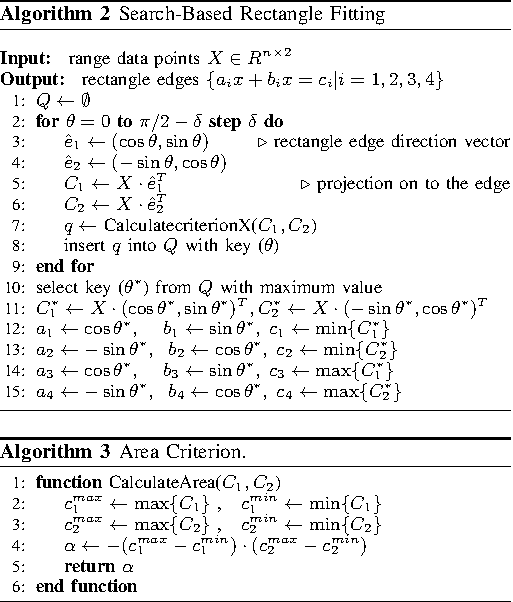
\includegraphics[width=0.49\linewidth]{figures/l_shape_fitting_fig_algs_1-cropped}
    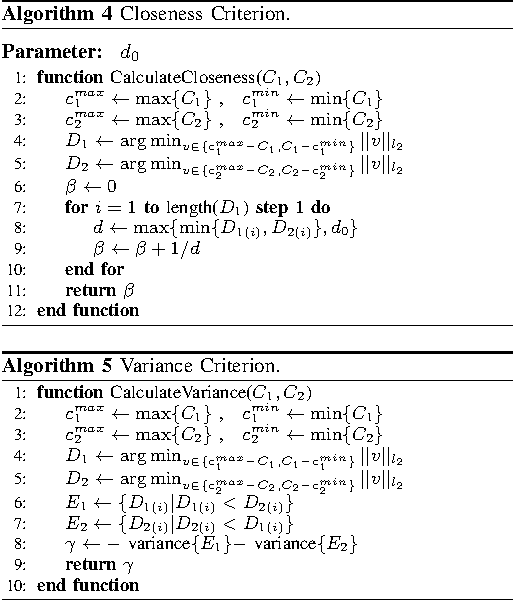
\includegraphics[width=0.49\linewidth]{figures/l_shape_fitting_fig_algs_2-cropped}
    \caption{Algorithms~2-5 from \textit{L-Shape-Fitting}~\cite{zhang2017efficient}. Algorithm~2 shows the main theta search loop, while Algorithms~3-5 are possible implementations of the \texttt{CalculateCriterionX} function.}
    \label{fig:lsf-algs}
\end{figure}

The algorithm uses a search-based approach (see Algorithm~2 of Figure~\ref{fig:lsf-algs}) to find the best-fit rectangle approximately.
It iterates through all possible directions of the rectangle and for each direction, it calculates the distances of all the points to the rectangle's four edges.
Based on these distances, the points are split into $P$ and $Q$, and the corresponding square errors are calculated as the objective function.
After iterating through all directions, the algorithm selects the optimal direction which achieves the least squared error, and fits the rectangle based on that direction.

The algorithm offers three different criteria for selecting the best-fitting rectangle: rectangle area minimization, points-to-edges closeness maximization, and points-to-edges squared error minimization.
Each criterion can be chosen to play the role of the \texttt{CalculateCriterionX} function in the algorithm provided in Figure~\ref{fig:lsf-algs}.
The choice of criterion depends on the specific requirements of the application.

The experimental results show that the algorithm is highly accurate and efficient, with a small mean and standard deviation of the estimation error.
Albeit computationally the most expensive, the variance criterion achieves the highest correctness, while the area minimization criterion sometimes fails to estimate the correct heading.

However, the algorithm may not always achieve perfect results.
For instance, the algorithm may fail to estimate the correct heading if the scan points are too sparse, or if there are points outside or inside of the L-Shape model.
Nevertheless, the impact of such imperfect cases on vehicle tracking can be minimized by biasing the algorithm's search space towards correct solutions using tracking and the HD map, as is done in this work.

% ----------------------------------------------------

\section{Evaluation Metrics}
\label{sec:evalmetrics}

Like in 2D object detection, the \textit{Average Precision (AP)} is also used as the main evaluation metric in 3D object detection.
The predictions are first assigned to their corresponding ground truths according to a specific similarity measure to compute AP\@.
The most commonly used similarity measure is the \textit{Intersection over Union (IoU)}, which is the geometric overlap between the ground truth 3D bounding box A and the estimated 3D bounding box B\@.
IoU is defined like this:

\[
\text{IoU}(A,B) = \frac{|A \cap B|}{|A \cup B|}
\]

The \textit{IoU} measure is used to judge a matched prediction as a \textit{True Positive (TP)} or a \textit{False Positive (FP)} by comparing it with a certain threshold.
Then, the recall $r$ and precision $p$ can be computed from the ranked detection results according to the following (FN denotes False Negatives):

\[
    r = \frac{\text{TP}}{\text{TP}+\text{FN}}, p = \frac{\text{TP}}{\text{TP}+\text{FP}}
\]

The precision can be regarded as a function of recall, i.e. $p(r)$: As recall approaches zero, the precision will rise, as there are fewer and fewer False Positives in the denominator.
Conversely, a rising recall is usually associated with a drop in precision, as the reduced amount of False Negatives leads to new False Positives.
The interpolated precision values across a range of recall values is defined as AP:

\[
    \text{AP} = \frac{1}{\mathbb{R}} \sum_{r \in \mathbb{R}} p(r)
\],

where the set $\mathbb{R}$ refers to a discrete set of values in practice.
The mean of this value across all object classes is called $mAP$.
The AP metric is commonly used to evaluate object detection performance, but it only considers the localization of objects and does not account for other factors such as dimension and orientation.
To address this limitation, \textit{nuScenes}~\cite{caesar2020nuscenes} proposed a set of True Positive (TP) metrics that measure other prediction errors from the true positives.

The five TP metrics are defined as positive scalars, including the \textit{Average Translation Error (ATE)}, \textit{Average Scale Error (ASE)}, \textit{Average Orientation Error (AOE)}, \textit{Average Velocity Error (AVE)}, and \textit{Average Attribute Error (AAE)}.
The \textit{ATE} measures the Euclidean distance between the object center on the 2D ground plane in meters.
The \textit{ASE} is the 3D Intersection over Union (IoU) error after aligning orientation and translation.
The \textit{AOE} is the smallest yaw angle difference between the predictions and ground truths in radians.
The \textit{AVE} is the absolute velocity error as the L2 norm of the velocity differences in 2D in meters per second.
Finally, the \textit{AAE} is defined as 1 minus attribute classification accuracy $(1-acc)$.

To obtain a single scalar score, \textit{nuScenes}~\cite{caesar2020nuscenes} computes the mean TP metric (mTP) over all object categories $\mathbb{C}$ for each TP metric using the following equation:

\[
    \text{mTP}_k = \frac{1}{\mathbb{C}} \sum_{c \in \mathbb{C}} \text{TP}_{k,c}
\]

where $\text{TP}_{k,c}$ denotes the k-th TP metric (e.g. $k=1$ means the ATE) for category $c$.
To integrate all the mentioned metrics into a scalar score, \textit{nuScenes} proposes the \textit{nuScenes} Detection Score (NDS) equation that combines the mAP and mTPk scores.
The NDS is calculated using the following equation:

\[
    \text{NDS} = \frac{1}{10} \left[5 * \text{AP} + \sum^5_{k=1}(1-\text{min}(1, \text{mTP}_k))\right]
\]

where AP is the mean average precision defined previously.
The term $1-\text{min}(1, \text{mTP}_k)$ is used to ensure that each TP metric contributes to the score positively, and the division by 10 is used to ensure that the score is in the range $[0, 1]$.

% ----------------------------------------------------
